\Chapter{Kínai karakterek felismerése}

{\large \textbf{Az alapvonások}}

Az írásjegyek felépítésének következő lényeges szabálya az írásjegy vonásainak sorrendje. Az írásjegyek – bármilyen bonyolult legyen is némelyik – tulajdonképpen néhány igen egyszerű vonalból épülnek fel. Ezek az írásjegyek alapelemei, vagy alap-ecsetvonásai. Az alábbi képen az alapvonások néhány főbb típusa látható. Természetesen az alapvonásoknak több változata is lehetséges (méret, vastagság, irány) attól függően, hogy az írásjegy melyik részén helyezkedik el.

\begin{center}
	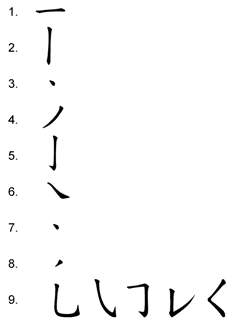
\includegraphics[width=0.4\linewidth]{images/chinese_strokes.png}
\end{center}

Minden egyes vonásnak megvan a felépítési szabálya: az ecsetvonásoknak meghatározott sorrendben kell követniük egymást, még pedig általános elvként az írásjegyek határait alkotó virtuális négyszög bal felső sarkából lefelé és jobbra haladva. Az írásjegy gerincét, fő szerkezeti elemét adó nagyobb vonást, ha az egész írásjegyet átjárja, legutoljára húzzák.

\newpage
{\large \textbf{A vonássorrend szabályai: }}
\begin{enumerate}
	\item A vízszintes vonások megelőzik a függőleges vonásokat.
	\item A balra lejtő vonások megelőzik a jobbra lejtő vonásokat. 
	\item Az írásjegyek írását felülről kell kezdeni. 
	\item Az írásjegyet balról jobbra haladva építik fel. 
	\item A felülről keretezett írásjegyeknél előbb a keretet kell meghúzni. 
	\item Az alulról keretezett írásjegyeknél a keretet legvégül kell meghúzni. 
	\item A teljes keretet mindig legvégül kell bezárni.
\end{enumerate}

Egy szimmetrikus felépítésű írásjegynél előbb a középső részt kell kialakítani, s csak azután az oldalakat.

\begin{center}
	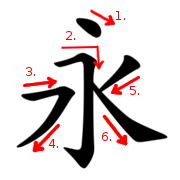
\includegraphics[scale=1.0]{images/vonasrend_ordered.png}
\end{center}

A kínai írásjegyek különböző számú alapvonásokból épülhetnek fel. Ezek közül a legegyszerűbb a csupán egyetlen vízszintes vonalból álló „egy” jelentésű \begin{CJK*}{UTF8}{gbsn}
一
\end{CJK*} ji írásjegy. A kínai írásrendszer más, egy vonásból álló írásjegyet nem tartalmaz. Aránylag ritkák a két vonásból álló írásjegyek is, például: \begin{CJK*}{UTF8}{gbsn}
二
\end{CJK*} er„kettő”,
\begin{CJK*}{UTF8}{gbsn}
十
\end{CJK*} si „tíz”,
\begin{CJK*}{UTF8}{gbsn}
人
\end{CJK*} zsen „ember” stb. A hagyományos írásjegyek zöme 15–30 vonásból épül fel (átlagosan 9 vonásból). Esetenként azonban ennél jóval több vonásból álló írásjegyek is előfordulhatnak, melyek tulajdonképpen már több önálló írásjegy összevonásának is tekinthetők. Ritkák ugyan, de léteznek 50 vagy akár 80 vonásból álló írásjegyek is.\\

{\Large OCR megvalósítások}\\

Az optikai karakterfelismerés feladata\\

A különböző formátumú dokumentumok kezelésének egyik speciális esete, amikor a kezelendő dokumentumok még nem állnak rendelkezésre elektronikus formában. Ebben az esetben szinte mindig arról van szó, hogy a dokumentumok kinyomtatva, papír alapú hordozón jelennek meg. Szövegbányászati tevékenység végzéséhez értelemszerűen digitalizálni kell a még nem digitalizált, papíron, nyomtatásban vagy írásban meglévő dokumentumokat, azaz a képként érzékelt dokumentumot szövegfájl formátumba kell átalakítani, hogy abban az után elektronikusan szerkeszthető és feldolgozható legyen. Ebben a szituációban kap szerepet az optikai karakterfelismerés (optical character recognition, OCR), amely így szövegbányászati előfeldolgozásnak tekinthető. Az optikai karakterfelismerés a mesterséges intelligencia jelfeldolgozó és generalizációs képességeit kiaknázva képes magas hatékonysággal nyomtatott, papír alapú dokumentumokon lévő karaktereket felismerni.

Az alap probléma itt az, hogy a nyomtatott papír alapú dokumentumok esetében nagy zajaránnyal kell megküzdeni annak érdekében, hogy a releváns információt kihámozzuk az érzékelt képi jelek és minták közül. Nyomtatott dokumentum esetében ilyen zajnak tekinthető például egy apró folt a papíron, tintaelmosódás, tintahiány, homályos háttér, apró gyűrodés a papíron, túl közeli vagy egybeolvadó betűk, betű dőlésszögének ingadozása stb. Kézírás esetén a kihívás még nagyobb, hiszen itt a személyiségjegyek sokszínűségéből adódó írásminták kavalkádjából kell kihámozni a karaktereket. Mind a nyomtatott, mind pedig a kézírásos esetben az optikai karakterfelismerő rendszer egy tanulási fázist követően képes olyanmintákat is osztályozni (a megfelelő karaktert felismerni), amelyekkel a tanulási fázisban nem találkozott, tehát megvan a szükséges generalizációs képessége.

Az OCR-rendszerek alapvetően két részből állnak: egyrészt a szkennelő fejből, amely a dokumentum egészét vagy részeit beszkenneli, másrészt pedig magából a mesterséges intelligencia szoftverből, ami elvégzi a beérkezett minták osztályozását, azaz magát a karakterfelismerést.

\begin{center}
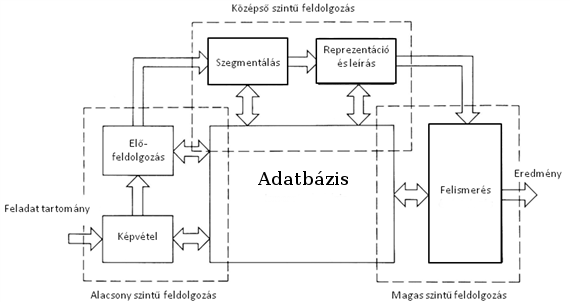
\includegraphics[scale=0.65]{ocr}
\end{center}

Szegmentáció

A szegmentáció során a karakterek közötti éles határ megtalálása a cél annak érdekében, hogy téves minták ne kerüljenek osztályozásra (pl. két fél karakter). A szegmentáció feladata lehet az is, hogy a karakter-dőlésszögeket, karakterméreteket normalizálja. Sok esetben a szöveges dokumentumokban nem csak karakterek vannak, hanem képek és egyéb, a felismerés szempontjából nem lényeges szimbólumok. A szegmentáció további feladata tehát az is, hogy az ilyen, számunkra nem releváns grafikus objektumok közül kiszűrje a csak karaktereket tartalmazó szöveges részeket.

\begin{center}
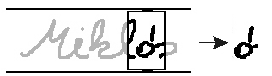
\includegraphics[scale=1.0]{ocr_segmentation}
\end{center}

Optikai előfeldolgozás

Az előfeldolgozás a bemeneti minta komplexitásának csökkentésére szolgál, és annak legjellemzőbb vonásait elemi ki. Különösen nagy jelentősége van a kézírás felismerésekor, ugyanis az írott betűk jóval komplexebb mintákat alkothatnak, mint a nyomtatott betűk. A jellemzőkiemelés során a komplexitás úgy csökken, hogy közben a legjellemzőbb információk megmaradnak és ezáltal a későbbi feldolgozás számításigényét redukálhatjuk. Ez a folyamat tulajdonképpen egy komplexitáscsökkentéssel járó digitalizáció. Az alábbi ábra egy egyszerű digitalizálási módszert mutat, amikor az analóg jelre egy mátrixot reprezentáló rácshálót illesztünk, és amelyik cellán átmegy az analóg karakter, az az elem a mátrixban 1 értéket vesz fel (fekete), egyéb esetben pedig 0-t (fehér).

\begin{center}
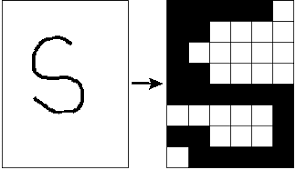
\includegraphics[scale=0.65]{ocr_preprocess}
\end{center}

Felismerés

Az osztályozás során történik meg a tényleges karakterfelismerés. A karakterfelismerő módszer a bemeneti jellemzővektor alapján dönti el, hogy az ismert karakterek közül melyikre hasonlít a legjobban a bemeneti vektor. Így a karakterfelismerési probléma egy asszociatív memóriát igénylő feladat, amelynek során a tárolt memóriaelemek közül kell előhívni azt, amely a bemeneti mintának legjobban megfelel.\\

Számjegyek felismerése zajos képeken\\

A következőkben bemutatok néhány olyan alkalmazást, amelyek az optikai karakterfelismerés egyes részeit hivatottak megvalósítani. Ezek között szerepelnek olyanok, amelyek meglehetősen szűk témakörrel, például számjegyek felismerésével foglalkoznak, de lesznek olyanok is, amelyek meglehetősen komoly eredményeket képesek felmutatni a kézírásos karakterek felismerése terén. Minden esetben részletesen kitérek arra, hogy az alkalmazás készítése során milyen megfontolások vezettek az adott neurális hálózat felépítésének megválasztásához, bemutatom az egyes területeken megjelenő és kezelendő problémákat, illetve összehasonlításokkal és adatokkal támasztom alá az egyes rendszerek hatékonyságát és alkalmazhatóságát a kijelölt problémára. 

A zajos számjegyek és karakterek a rendszámtáblák felismerésénél általános jelenségnek számítanak, mivel itt a kamera felvétele általában mozgó járműről készül, és a zajt tovább növelheti a piszok, a nedves, esetleg esős időjárás, éjszakai sötétség, a tükröződés stb.

Jelen esetben tekintsünk el a különböző felvételi körülmények által okozott természetes hibáktól és vizsgáljuk meg, milyen eredménnyel ismerünk fel mesterségesen eltorzított képeken számjegyeket. A beolvasott képeket a következő módszerekkel tesszük zajosabbá: 

\begin{itemize}
\item Gauss zajok alkalmazásával. 
\item Képfeldolgozási eszközök használatával (elmosás). 
\item Véletlenszerűen részletek kitörlésével. 
\end{itemize}

Mivel a program hatékonyságát nagymértékben befolyásolja a neurális hálózat felépítése, gondosan meg kell tervezni, hogy milyen hálózatot alkalmazunk az egyes problémák megoldásához. Jelen esetben az átlagos négyzetes hiba (MSE) segítségével értékeljük a hálózat hatékonyságát és több hálózat teljesítményét összevetve választjuk ki, hogy milyen felépítést használunk a jelenlegi problémánkhoz. 

Első lépésben ki kell választanunk a rejtett és a kimeneti réteg neuronjai által alkalmazott aktivációs függvényt. Jelen esetben a rejtett rétegbeli neuronoknál tangens szigmoid, a kimeneti réteg neuronjainál pedig logaritmus szigmoid függvényt alkalmazunk. 

Természetesen lehetőségünk lenne akár minden rejtett rétegbeli neuronnál, illetve minden kimeneti neuronnál ugyanazt vagy akár mindegyiknél különböző aktivációs függvényt használni, de jelen esetben, a négyzetes hiba mértékét figyelembe véve ez a két függvény megfelelőnek látszik arra, hogy a segítségével a neurális hálózatunk nagy hatékonysággal ismerje fel az egyes számjegyeket.

Szintén próbálgatásos módszer segítségével a rejtett neuronok számát 9-ben határoztuk meg. Rögzített 50 tanítási epoch mellett a legkisebb négyzetes hibát adó rejtett rétegbeli neuronszámot választottuk.

A következő táblázatból látszik, hogy nem lehet egyértelműen megmondani, hogy az egyes neuronszámok mellett milyen hibaértékek várhatók. A táblázatból az is kitűnik, hogy 9 rejtett neuronnal a négyzetes hibát látványosan kisebbre lehetett visszaszorítani. 

\begin{center}
\begin{tabular}{ |c|c|c| } 
 \hline
 Rejtett neuronok száma  & MSE  \\ 
 \hline\hline
 1 & 0,1424 \\
 \hline
 2 & 0,0485 \\
 \hline
 3 & 0,0508 \\
 \hline
 4 & 0,0745 \\
 \hline 
 5 & 0,0809 \\
 \hline
 6 & 0,0933 \\
 \hline
 7 & 0,1183 \\
 \hline 
 8 & 0,0386 \\
 \hline
 9 & $1,9509*10^{-12}$ \\
 \hline
 10 & 0,0039 \\
 \hline
 11 & 0,1691 \\
 \hline
 12 & 0,0025 \\
 \hline
 13 & 0,0014 \\
 \hline
 14 & 0,0014 \\
 \hline
\end{tabular}
\end{center} 

A neurális hálózat ideális felépítésének meghatározása után a következő lépés a tanulóhalmaz összeállítása. A számjegyek felismerésére készített hálózatot a következő tanulópéldákkal tanítjuk be: 

\begin{itemize}
\item Normál számok 
\item Háromszor és tizenkétszer elmosott számok 
\item Öt és harminc közötti intenzitású Gauss zajjal módosított számok
\end{itemize}

A normál számokat 100\%-ban, az elmosott számokat átlagosan 95\%-ban, a Gauss zajjal kezelt számokat átlagosan 94\%-ban ismerte fel.

Nyomtatott karakterkészlet

Ebben a részben két speciális betűtípussal nyomtatott karakterek felismerését tekintjük át egy neurális hálózatot alkalmazó program működésén keresztül. Mindkét betűtípus 84 karaktert tartalmaz, a karakterek pedig 8 x 8-as felbontásúak.

A számjegyek felismerésének problémája látványosan egyszerűbb, mint az általános karakterfelismerés által támasztott feladat. Első lépésként vizsgáljuk meg, hogyan és milyen hatékonysággal ismerhetünk fel nyomatott karaktereket.

A feladat megoldásához használt hálózatban 64 bemeneti neuront alkalmazunk. A hálózat általános előrecsatolt neurális háló. A 64 bemeneti neuron mindegyike a 8 x 8-as karakter egy-egy pixeléhez van kötve. A bemenet fekete pixelek esetén 1, egyéb esetekben 0 értékű.

Mivel a neurális hálózatok hatékonysága nagymértékben függ a hálózat méreteitől, elmondhatjuk, hogy a fenti módszerrel felépített hálózattól nem várhatunk túlságosan hatékony működést. Természetesen egy ilyen hálózat is betanítható oly módon, hogy szembetűnő eredményeket mutasson fel, de ehhez lényegesen több erőforrásra és időre van szüksége, mint az előző példában bemutatott, jóval kisebb hálózatnak.

A rendszer teljesítményének meghatározásához először külön-külön, aztán összesítve is megvizsgáljuk a két választott karakterkészletből vett minták felismerési arányát. Az értékelésnél külön vesszük a rendszer által ismeretlennek titulált és a rosszul felismert karaktereket.

A két karakterkészlet összesített eredményeiből levonhatjuk azt a következtetést, hogy egy neurális hálózat számára valóban jóval nagyobb nehézséget jelent, ha nem „tudja”, hogy pontosan milyen karakterekre számítson. Ez a feladat már előrevetíti, hogy milyen nehézségekkel kell szembenéznünk, ha nem egy fix karakterkészletből választott betűket akarunk a rendszerünkkel felismertetni, mint ahogy ez a kézzel írt karakterek esetében is történik. Mindemellett a különböző betűkészletből vett nyomtatott karakterek felismerése annyiban tűnhet egyszerűbbnek, hogy ha fix számú betűtípust használunk, akkor még mindig tekinthetjük úgy, hogy fix karakterkészlettel van dolgunk és elégséges a hálózatnak minden betűtípusból egy-egy mintát megtanítani az egyes betűkből.

\begin{center}
\begin{tabular}{ |c|c|c| }
\hline
\multicolumn{3}{|c|}{\textbf{Összesített eredmények}}\\
\hline
Felismert karakterek & 99 db & 54\%\\
\hline
Ismeretlen karakterek & 5 db & 3\%\\
\hline
Rosszul felismert karakterek & 64 db & 38\%\\
\hline
Összes ismeretlen vagy rosszul felismert karakter & 69 db & 41\%\\
\hline
\end{tabular}
\end{center}


Kézzel írt karakterkészlet

Az előbbi két példából látszik, hogy a számjegyek felismeréséhez képest a tetszőleges nyomtatott karakterek felismerése jóval nehezebb feladat még abban az esetben is, ha csak limitált számú, megadott betűtípusokból vesszük a bemeneti adatokat. A kézírásos karakterek felismerése még ennél a pontnál is jóval tovább megy, hiszen gyakorlatilag nem támaszkodhatunk arra, hogy egy adott karakterkészletből kell kiválasztanunk a megfelelő betűt.

A kézírások változatosságából adódóan nagyon körültekintően kell megválasztanunk, hogy milyen módszert, illetve milyen felépítésű neurális hálózatot használunk, hiszen nem csak a felismerés hatékonyságát, hanem a rendszer betanítási és futási idejét is figyelembe kell
vennünk.

Ebben a részben egy olyan neurális háló alkalmazással ismerkedünk meg, amely már kézzel írt karaktereket kap bemenetként és ezek felismerésére tesz kísérletet. 

A kézzel írt karakterek felismerésének első lépéseként a felismerni kívánt karaktereket szeparálni kell a képen található többi információtól, illetve a szavakat, szókapcsolatokat karakterekre kell bontani. A kép ilyen formájú feldolgozása után az egyes karaktereket tartalmazó képeket digitalizálni kell. A digitalizálás folyamán a képekből egy bináris mátrix készül. Minden fekete pixelnek egyest, minden fehérnek nullát feleltetünk meg. 

A következő ábrán látható, hogy milyen lépések folyamán jutunk el a kézzel írt A betűtől addig a bitmátrixig (I), amelyet a neurális hálózat már értelmes bemenetként képes kezelni. A digitalizálás folyamán minden karaktert ugyanakkora méretűvé alakítunk, így a hálózat minden esetben egy előre meghatározott méretű bitmátrixszal dolgozik majd. 

\begin{center}
	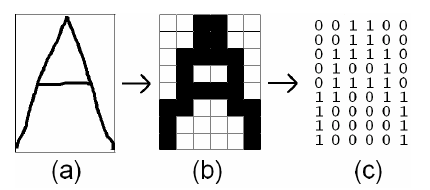
\includegraphics[scale=0.75]{HandwrittenA}
\end{center}

A karaktereket ennél a programnál felügyelt tanulással tanítjuk be a rendszernek. Minden karakterhez tartozik egy \textit{címke}, amely azt határozza meg, hogy az adott kép milyen betűt reprezentál. Minden címkéhez számos karaktert használunk fel a tanítási folyamat során, így a rendszer többféle variációban is "látja" az egyes betűket. A tanításhoz egy \textit{M} bemeneti mátrixot használunk.

A \textit{k}-adik megtanulandó karakterhez tartozó súlymátrixot \(W_k\)-nak nevezzük. Ez a mátrix alapértelmezés szerint nullmátrixként van inicializálva. A súlymátrix változtatására egy egyszerű algoritmust használunk.

\begin{lstlisting}[language=Python]
for i in range(1, x):
	for j in range(1, y):
		W[i][j] = W[i][j] + M[i][j]
\end{lstlisting}

Ezt az algoritmust minden egyes tanulópélda esetén lefuttatjuk, ezáltal kialakítjuk a neurális hálózatban a felismeréshez használt súlyokat.

Példaként tekintsük meg az S betű három eltérő előfordulását és vizsgáljuk meg az S betűhöz tartozó súlyvektort a tanítási fázis után.

\begin{center}
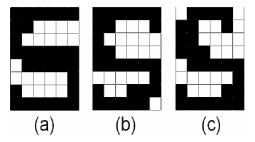
\includegraphics[scale=0.75]{ocr_S}
\end{center}

Az ábrán látható, hogy az S betűt többféle módon is le lehet írni. Ezek közt a betűk közt az emberi agy ugyan érzékeli a különbséget, azonban elmondható, hogy még ennél sokkal nagyobb eltérések esetén is képesek lennénk felismerni egy S betűt.

Ha jobban megfigyeljük a betűket, észrevehetjük azokat a szemmel látható hasonlóságokat, amelyek alapján az agyunk megállapítja, hogy ezek a képek S betűket ábrázolnak. Ha egy S betűt magunk elé képzelünk, mindenképpen egy jobb felső sarokból induló görbét látunk, amely valahol középen irányt változtat és a bal alsó sarokban fejeződik be. Az ábrán látható három S betű magán viseli ezeket a jellegzetességeket, habár ezeket konkrét reprezentáció esetén csak nehezen tudjuk leírni. A korábban leírt tanítási algoritmus során a súlyvektorban kiemeljük azokat a részeket, amelyek leghangsúlyosabbak az egyes karakterek előfordulásainál.

A rendszerben használt hálózat bemenete egy bitmátrix (tanulópéldák esetén M). A bemenetet n darab különböző karakter felismerésének tanítása esetén n darab neuronnak adjuk át.

A vizsgált S betű egyik megtanult S mintával sem mutat teljes egyezőséget, a hálózat mégis 0,68-as felismerési hányadost számolt ki hozzá, amelynél már megállapíthatjuk az egyezést.

Ha ugyanennyi tudással rendelkező rendszerünknek egy másik betűt, mondjuk egy P-t adunk meg bemenetként, abban az esetben a felismerési hányados jóval kisebb (0,21) lesz, tehát a csupán S betűket ismerő rendszer biztosan nem fogja felismerni.

A rendszer tudásbázisa könnyedén bővíthető új karakterek, illetve a már megtanult karakterek újabb változatainak megtanításával. Maga a rendszer meglehetősen általános és a karakterek méretére és arányaira invariáns.